\documentclass[12pt,oneside,draft]{fithesis2}
\usepackage[czech]{babel} % package for multilingual support
\usepackage[utf8]{inputenc}
\usepackage[T1]{fontenc}
\usepackage[plainpages=false,pdfpagelabels,unicode]{hyperref}
\usepackage{graphicx}
\usepackage{natbib}
\usepackage{longtable}
\usepackage{pdfpages}
\usepackage{mathtools}

% citation style and punctuation
\bibpunct[: ]{(}{)}{,}{a}{}{;}

% czech quotes
\usepackage{csquotes}
\DeclareQuoteStyle{czech}
  {\quotedblbase}
  {\textquotedblleft}
  {\textquoteleft}
  {\textquoteright}

\renewcommand{\uv}[1]{
  \enquote{#1}
}

\thesistitle{Institucionální design grantové komise na principech deliberace \emph{(případová studie)}} % enter thesis title
\thesissubtitle{diplomová práce}
\thesisstudent{Jan Martinek}    % name of the author
\thesiswoman{false} % defines author’s gender
\thesisfaculty{fss}
\thesisyear{jaro 2013}
\thesisadvisor{doc. PhDr. Ing. Ondřej Císař, Ph.D.} % fill in advisor’s name
\thesislang{cs}

\begin{document}
\FrontMatter
\ThesisTitlePage

\begin{ThesisDeclaration}
\DeclarationText
\AdvisorName
\end{ThesisDeclaration}

\begin{ThesisDedication}
\vspace*{10cm}
\noindent
\emph{Věnováno památce Anny Matušinové, \newline první předsedkyně Stipendijní komise.}
\end{ThesisDedication}

\begin{ThesisThanks}
Rád bych poděkoval..., Císař, tým GoodReader, rodiče, anonymní rozhovoranti, čteči [], FSS, sociologové, Falk, Karel Musílek, SublimeText, John MacFarlane - Pandoc, Markdown, LaTeX, Proof \& Reason a HejTi, Vojta Šmíd a Karel Gargulák, Vendula Venclíková, vyučující, kteří mě silně ovlivnili (viz kapitola 3)
\end{ThesisThanks}

\begin{ThesisAbstract}
Abstrakt...
\end{ThesisAbstract}

\begin{ThesisKeyWords}
keyword1, keyword2, etc.
\end{ThesisKeyWords}

\MainMatter

\tableofcontents          % prints table of contents

\chapter{Další kapitola}
...

\chapter{Úvod}

První kapitola… pokus...

\chapter{Jiná kapitola}

\bibliographystyle{apa-good}
\bibliography{sources}

% prilohy
\chapter{Příloha A: Pravidla fungování komise sepsaná Studentskou komorou AS}
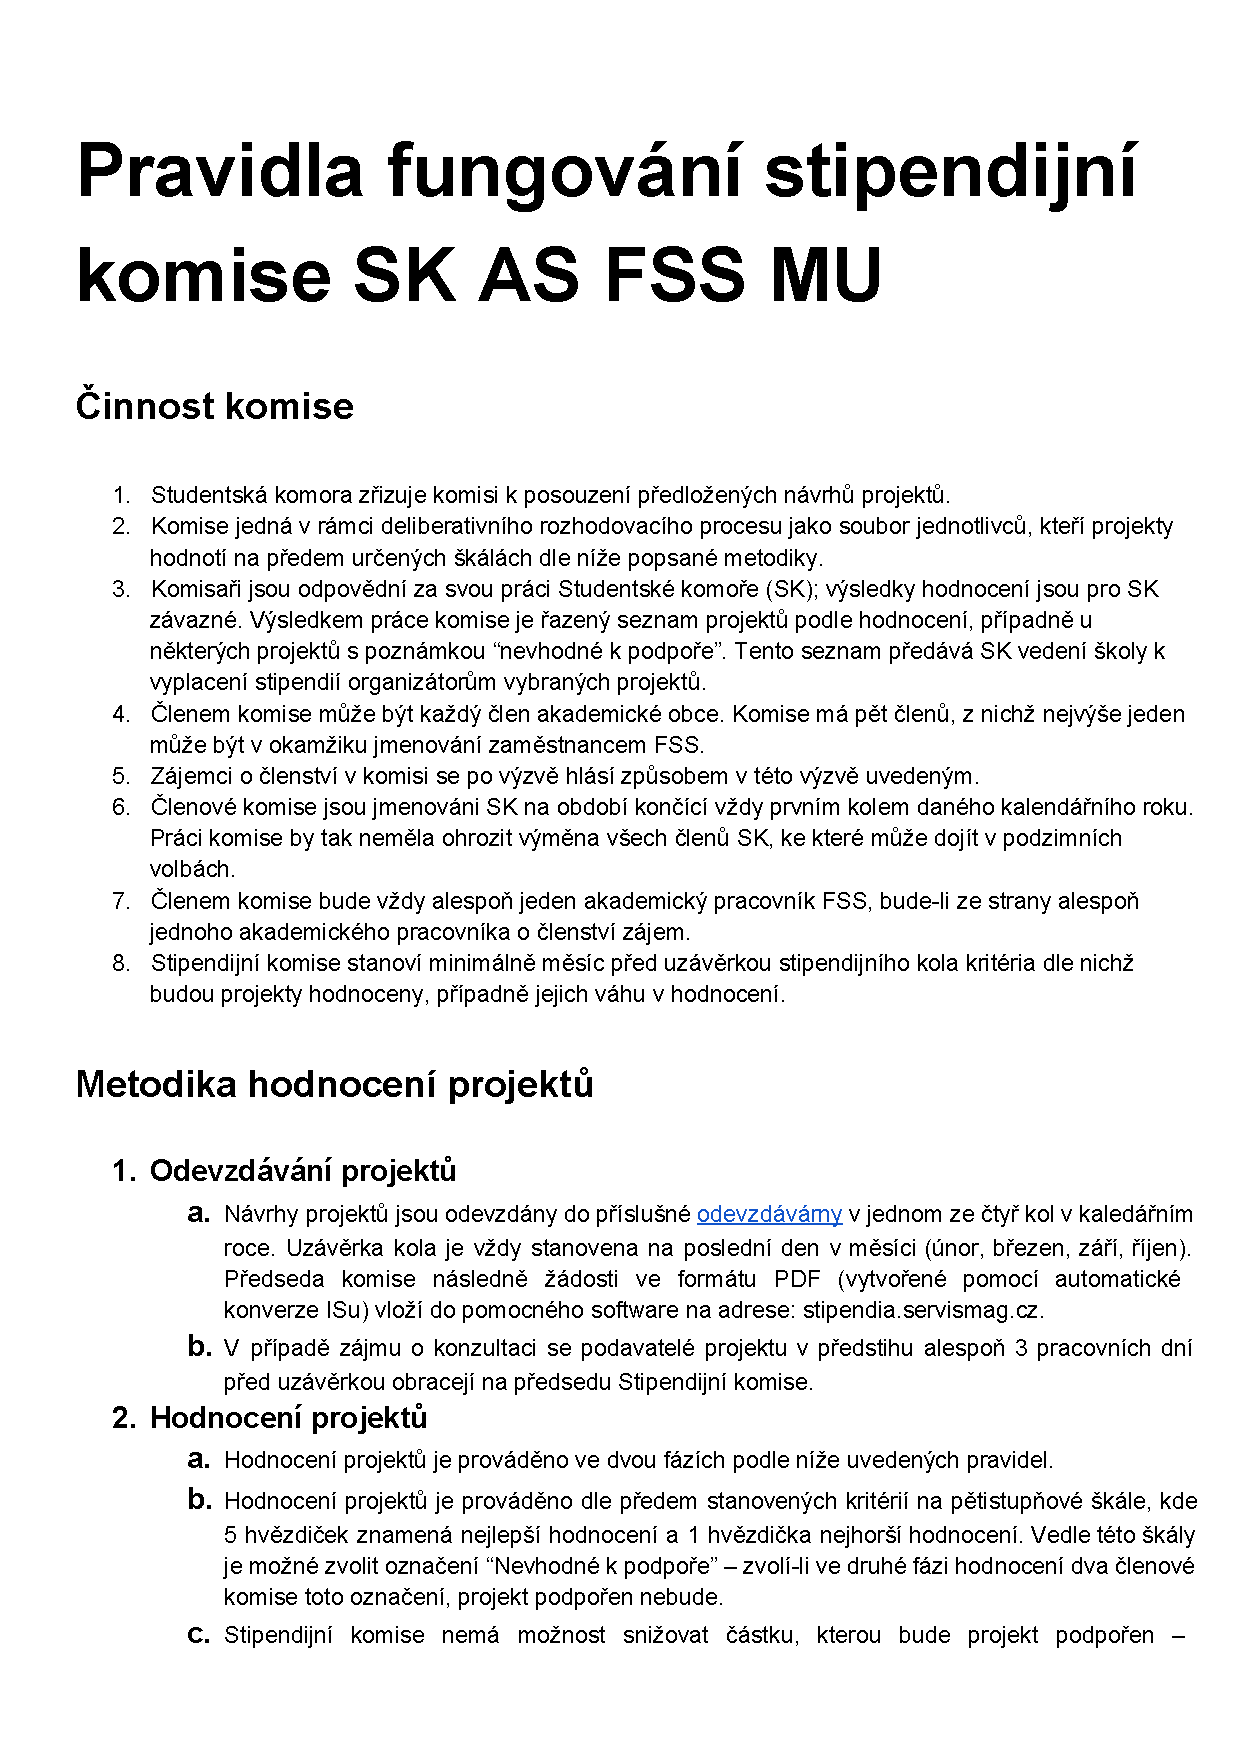
\includepdf[pages={1,2}]{pravidla-fungovani-prvotni-verze.pdf}

\chapter{Příloha B: Pravidla fungování komise upravená Stipendijní komisí}
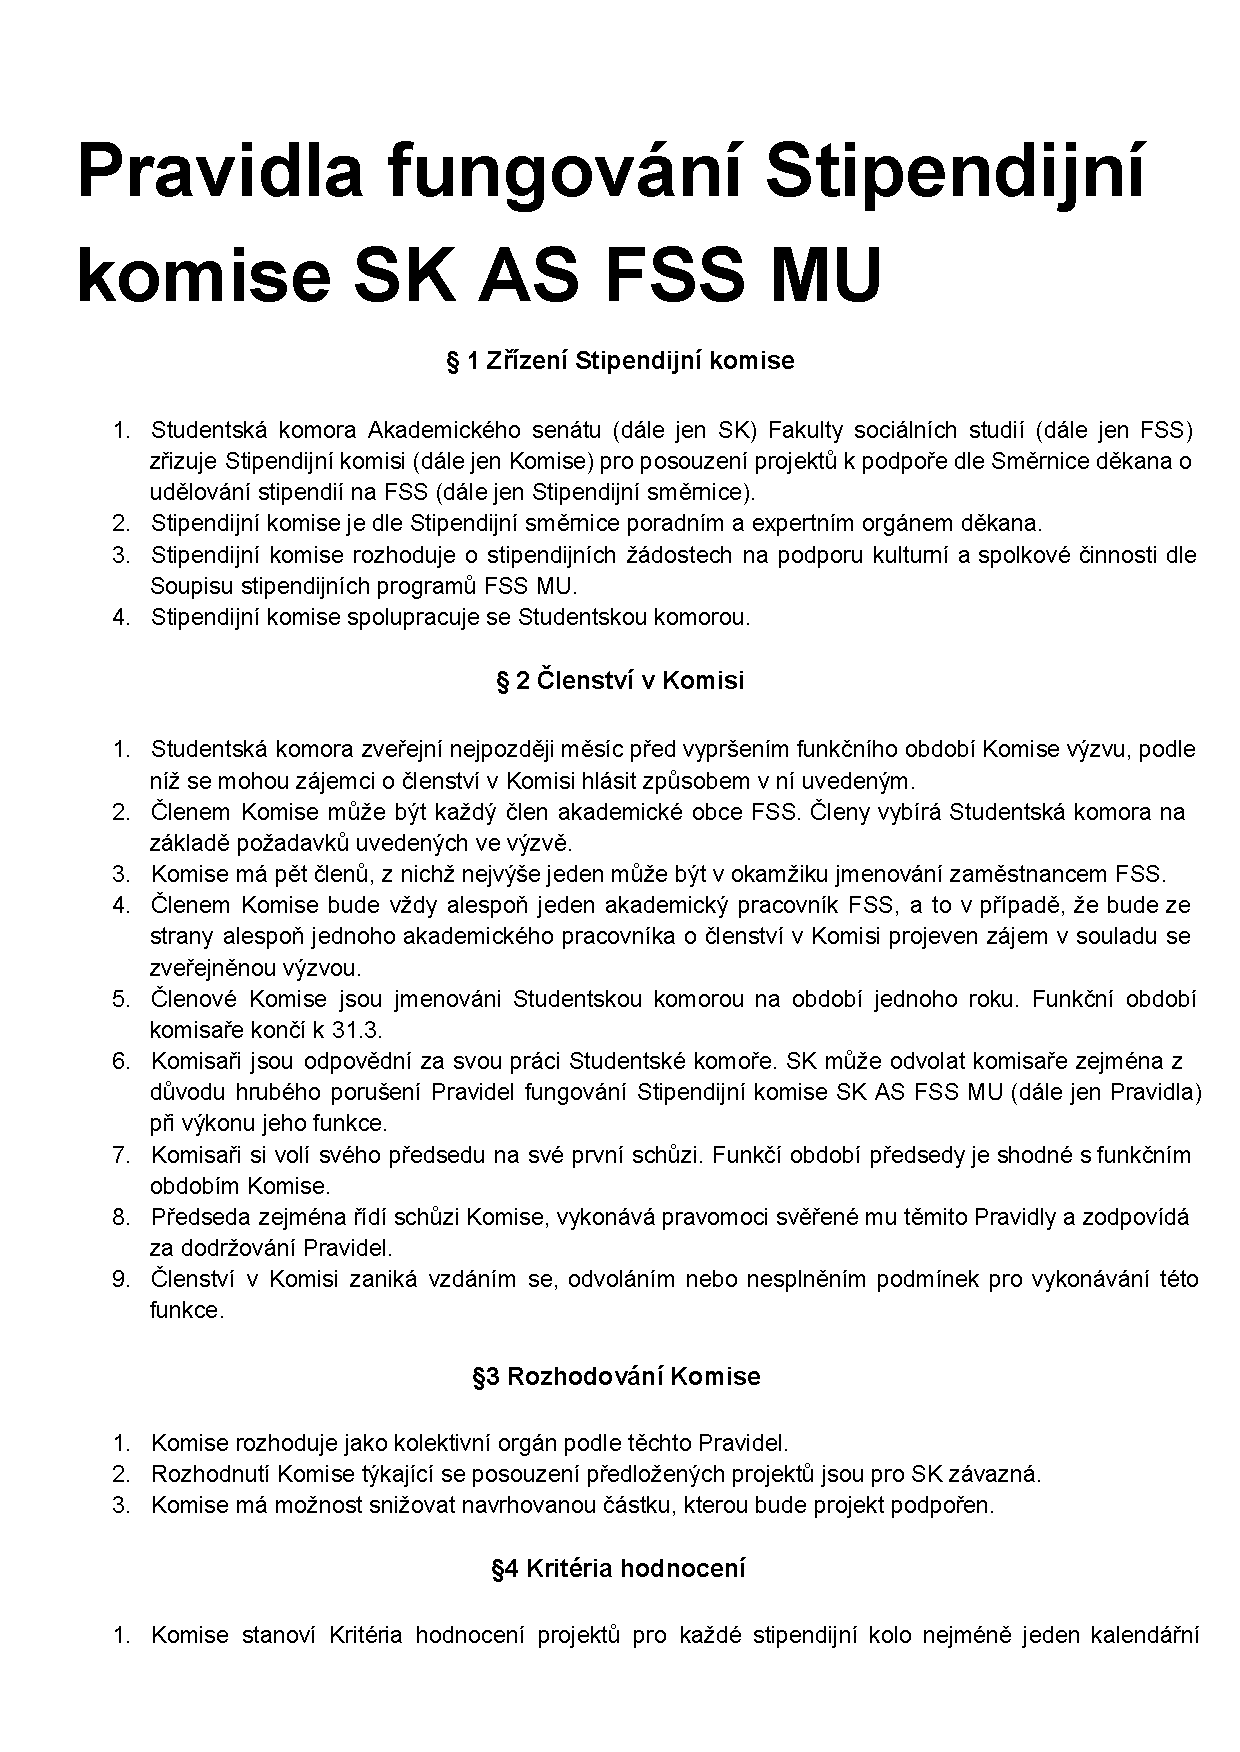
\includepdf[pages={1,2,3,4}]{pravidla-fungovani-konecna-verze.pdf}

\end{document}